\documentclass[../main.tex]{subfiles}
\begin{document}

\chapter{Grundlagen}
\label{basics}

	\section{Virtualisierung}
  \label{introVirt}
    Bei der Virtualisierung, deren Anfänge sich auf IBM-Forschungsprojekte von 1964 zurückführen lassen, werden ein oder mehrere virtuelle Systeme auf einem physischen System betrieben. Virtuelle und physische Systeme können dabei als minimale oder vollständige Betriebssysteme vorliegen. Systeme können in Rechenzentren eine Serverinfrastruktur bilden, in der virtuelle als auch physische Komponenten gemeinsam verwaltet werden \cite[S.661]{tanenbaumOS}.

		Zunächst werden Formulierungskonventionen und ein Wortschatz definiert, die grundlegende Merkmale der Virtualisierung einführen und im Rahmen dieser Arbeit zum Verständnis beitragen sollen.

		Die Unterscheidung in \glqq{}virtuelle\grqq{} und \glqq{}physische\grqq{} Systeme ist nicht von Bedeutung, wenn allein der Begriff \glqq{}System\grqq{} aufgeführt ist. Wenn die Abgrenzung minimaler Betriebssysteme von vollständigen Betriebssystemen notwendig ist, wird das jeweilige Attribut an entsprechender Stelle verwendet. Standardmäßig ist allgemein von einem (Betriebs-)System die Rede. Per Definition in dieser Arbeit, besteht ein System aus mindestens einem Betriebssystem und zugehörigen Peripheriegeräte, wie z.B. einem Netzwerkanschluss.

		Ein System, das in der Rolle eines Wirts mehrere virtuelle Systeme betreibt, wird allgemein als Host oder Hostsystem bezeichnet. Systeme, die einzeln oder parallel virtualisiert auf einem solchen Host laufen, werden als (virtuelle) Gastsysteme bezeichnet.

		Der Begriff des Hosts ist abzugrenzen von der Bedeutung eines Hosts in der Netzwerktechnik. In der Netzwerktechnik ist damit ein kommunikationsfähiger Netzwerkknoten gemeint. Der in dieser Arbeit mehrfach erwähnte Host meint das Betriebssystem, welches Gastsysteme startet und stoppt.

		Das Hostsystem kann physischer oder virtueller Natur sein:
		\begin{itemize}
			\item \textbf{Physischer Host}: Hostsystem, das Gastsysteme verwaltet und selbst direkt (nativ) auf der Hardware läuft.
			\item \textbf{Virtueller Host}: Hostsystem, das Gastsysteme verwaltet und selbst als Gastsystem eines übergeordneten Hosts existiert.
		\end{itemize}

		Im Vergleich zu dieser Unterscheidung ist ein Gastsystem immer virtueller Natur. Die Einheit eines physischen Hosts inklusive aller darin betriebenen virtuellen Systeme, wird in dieser Arbeit als Maschine bezeichnet.

		Wie der Begriff \glqq{}Virtueller Host\grqq{} andeutet, sind virtuelle Verschachtelungen in der Architektur von Maschinen möglich und auch in der Praxis bis zu einem gewissen Grad sinnvoll. Beispielsweise kann in einem Rechenzentrum, jeder physische Host von mehreren Kunden verwendet werden, indem jedem Kunden eine Gastsystem auf diesem physischen Host zugewiesen wird. Ein Kunde kann dieses Gastsystem wiederum als virtuellen Host betreiben, das jede Anwendung des Kunden in einem eigenen, neuen Gastsystem virtualisiert. Wie diese Trennung von Kunden und Kundenanwenddungen zeigt, eignet sich eine Verschachtelung der Systeme zur Abbildung von logischen Strukturen.

		% --- schnitt ----

		Virtualisierte Systeme nutzen im Vergleich zu nativen (physischen) Systemen zusätzliche Software, die den virtualisierten Systemen in der Ausprägung von virtuellen Maschinen, sogenannte \acrshort{VM}s, und Containern, mehrere Abstraktionen anbietet, um Funktionen des Hostsystems abzubilden \cite[S.2]{containerVirtPerformance}. Beide Ausprägungen erwecken aus Sicht des Gastsystems den Eindruck, dass ein alleinstehendes Betriebssystem ausgeführt wird.
    Der Einsatz von Virtualisierung bietet vielfältige Vorteile für \acrshort{IT}-Unternehmen. In der folgenden Auflistung sind einige Problemfaktoren und Anforderungen an Rechentzentren und darin laufender Software zusammengefasst, die alle durch Virtualisierungslösungen addressiert werden können \cite[S.1]{bsiVirt}\cite[S.662,672f.]{tanenbaumOS}\cite[S.299]{mandlOS}.

		% \multicolumn{1}{l|}{
		\begin{table}[htp]
			\begin{centering}
		  %\begin{tabular}{ | l | l | }
			\begin{tabularx}{\textwidth}{>{\hsize=1\hsize}X>{\hsize=1\hsize}X}
				\hline
				\textbf{Herausforderung} & \textbf{Lösungsansatz mithilfe von Virtualisierung} \\
				\hline
				Rechenzentren sollen möglichst effizient betrieben werden, da anfallende Energiekosten für den Betrieb und die Kühlung von Servern auch bei geringer Auslastung anfallen.
				& Kosteneinsparungen bei der Anschaffung von Hardware und Lizenzen sowie dem Energieverbrauch möglich, da virtuelle Instanzen die physischen Ressourcen effizienter ausnutzen können und demnach in Summe auch weniger physische Maschinen benötigt werden. \\
				\hline
				Softwarelösungen sollen skalierbar sein. Je nach Bedarf sollen Kapazitäten in der IT-Infrastruktur freigeschalten oder reduziert werden können.
				& Die Virtualisierung ermöglicht es, hardwareunabhängige, portierbare und reproduzierbare Softwarekomponenten zu realisieren, die flexibel aktiviert und deaktiviert werden können. \\
				\hline
				In einem Rechenzentrum wird Software unterschiedlicher Kunden ausgeführt (Multi-Tenancy-Umgebung). Eine Trennung dieser Kundeninstanzen muss gewährleistet sein, sodass diese nicht miteinander interferieren können.
				& Virtuelle Lösungen bieten verschiedene native Möglichkeiten zur Isolierung von Systemen. Eine Gefahr von Interferenz zwischen Kunden kann je nach eingesetzer Technologie auf unterschiedliche Art und Weise reduziert werden. \\
				\hline
				Redundanz, um Ausfällen entgegenzuwirken, soll gewährleistet sein.
				& VMs und Container sind flexibel zu starten und stoppen. Ausfallsicherheit wird in Form mehrerer redundanter virtueller Instanzen und der Unterstützung von Tools ermöglicht. \\
				\hline
				Bestimmte Architekturen, wie z.B. 3-Tier-Architektur, sollen komfortabel umgesetzt werden.
				& Einzelne Bausteine beliebiger Architekturen lassen sich mit virtuellen Instanzen unabhängig voneinander betreiben und vernetzen. \\
				\hline
				Über die Zeit hinweg entstehen unterschiedliche Softwareversionen, die ggf. von teils alten Anwendungen und Bibliotheken abhängen. Die verschiedenen Versionen sollen zuverlässig und unabhängig voneinander betrieben werden. Nicht nur Anwendungen, sondern auch Betriebssysteme unterschiedlicher Art sollen ggf. möglichst hardwareunabhängig einsetzbar sein.
				& Virtualisierungen bieten gute Migrationseigenschaften und sind mit einer Vielzahl von Betriebssystemen kompatibel. Vor allem die containerbasierte Virtualisierung erlaubt einen hohen Grad an Modularisierung und Kompatibilität. Produkte werden können nicht nur als Programme vertrieben, sondern als plattformunabhängige \emph{Virtual Appliances}, also in virtuelle Instanzen eingebettete Anwendungen \cite[S.672f.]{tanenbaumOS}. \\
				\hline
				Neue Services und Kunden sollen einfach in bestehende Infrastrukturen integrierbar sein. Systeme sollen einfach kombinierbar und zwischen Rechenzentren portierbar sein.
				& Virtuelle Instanzen können als sogennante Snapshots \glqq{}eingefroren\grqq{} werden und in anderen Infrastrukturen wieder fortgefahren werden.\\
			  \hline
				Gute Administrationsmöglichkeiten und Wartbarkeit der Infrastruktur
				& Virtualisierte Systeme lassen sich neben physischen Systemen zusammen, ggf. an zentralisierter Stelle, verwalten. Eine gleichzeitige Senkung der Administrationskosten ist möglich \cite[S.1]{bsiVirt}.
		  \end{tabularx}
			\caption{Mehrere Herausforderungen im Betrieb von IT-Infrastrukturen und deren Lösungsansatz mithilfe von Virtualisierung}
			\end{centering}
			\label{tab:virtAdvantages}
		\end{table}
		% TODO: Tabelle ist leider abgeschnitten

		Wie in Tabelle \ref{tab:virtAdvantages} zu sehen ist, bietet der Einsatz von serverseitiger Virtualisierung eine Reihe von Vorteilen, die ein rein physischer Betrieb von Servern nicht in dem Maß bieten kann. Diese Vorteile eröffneten IT-Unternehmen auch neue Geschäftsmodelle, auf denen der Erfolg von heutigen Cloud-Anbietern wie \emph{Amazon}, \emph{Google} und \emph{Microsoft} beruht. Selbst einhergehende Nachteile der Virtualisierung, wie z.B. Leistungsverluste und in dieser Arbeit untersuchte Sicherheitsrisiken, scheinen, den Vorteilen gegenübergestellt, nicht ins Gewicht zu fallen.

		Im Folgenden sind die Konzepte der Virtualisierung auf Hypervisor- und Containerbasis erklärt und in ihren ausschlaggebenden Eigenschaften gegenübergestellt.

		%% TODO: folgendes integrieren im text von introVirt .... UPDATE: schon teils geschehen 2 abseatze drueber
	  %Sowohl Hypervisor-gestützte VMs als auch Container erwecken aus Sicht des Gasts den Eindruck, dass ein alleinstehendes Betriebssystem ausgeführt wird (QUELLE: “OpenVZ,” 2012. [Online]. Available: http://www.openvz.org). Um diese Illusion zu schaffen, wird jedoch wie beschrieben jeweils ein anderer Ansatz eingesetzt.

		% TODO: cahpter 2 usage scenarios einbinden aus
		%	Evtl. auch strengere Trennung in verschiedene Vorteile von Virtualisierung.
		%		^		\cite[S.2,3]{dockerSec2}

    \subsection{Hypervisor-basierte Virtualisierung}
    \label{introVirtHypervisor}
      Im Kontext einer Hypervisor-basierten Virtualisierung wird das virtuelle System eine \acrshort{VM} genannt. \acrshort{VM}s enthalten jeweils eine Umgebung, die Abstraktionen eines sogenannten Hypervisors nutzt, um Hardwareressourcen des Hosts zu verwenden. Der Hypervisor, auch seltener \emph{Virtual Machine Monitor} (\emph{VMM}) genannt, ist ein Stück Software, das zwischen einem Host- und einem Gast-Betriebssystem (der \acrshort{VM}) vermittelt und Hardwareabstraktionen des ersteren bereitstellt \cite[S.6]{dockerBook}\cite[S.2]{containerVirtPerformance}\cite[S.2]{dockerSec1}. Ein weitere wichtige Eigenschaft eines Hypervisors ist es, dem Gast jede für den Betrieb eines Betriebssystems nötige Funktion anzubieten \cite[S.106]{tanenbaumOS}

      % Auf dieser Art von Systemen laufen eine oder mehrere VMs unabhängig voneinander auf physischer Hardware (in der englischen Literatur auch "bare metal" genannt). Der Hypervisor, der auch \emph{Virtual Machine Monitor} (\emph{VMM}) genannt wird \cite[S.2]{containerVirtPerformance}, nimmt dabei die Rolle eines Vermittlers zwischen Host-OS und Gast-OS ein \cite[S.6]{dockerBook} und abstrahiert dem Gast das komplette Funktionsset des Hosts. \cite[S.2]{dockerSec1}.

      Durch diese Technik läuft in jeder \acrshort{VM} ein eigenes (Gast-)Betriebssystem, das von solchen anderer \acrshort{VM}s isoliert läuft. Durch die Abstraktion des zwischenliegenden Hypervisors ist es möglich, mehrere unterschiedliche Gastbetriebssysteme auf einem physikalischen Host auszuführen \cite[S.2]{containerVirtPerformance}\cite[S.106]{tanenbaumOS}.

			Trotz der in Tabelle \ref{virtAdvantages} aufgeführten effizienteren Ressourcennutzung im Rahmen von Virtualisierungstechniken, stehen Hypervisor heute unter dem Ruf ineffizient zu arbeiten. Dieser größte Kritikpunkt der genannten Virtualisierungsmethode, lässt sich auf den Erfolg der containerbasierten Virtualisierung zurückführen, die, wie in Kapitel \ref{introVirtContainer} weiter ausgeführt, weniger Overhead erzeugen.
			% TODO: Overhead ins Glossar?

      Hypervisortechnologien werden in solche von Typ 1 und Typ 2 unterschieden:

			Der Typ 1 Hypervisor operiert direkt auf der Hardware des Hosts und stellt ein minimales, speziell für den Betrieb von VMs ausgelegtes Betriebssystem dar. Dessen Aufgabe ist es, Kopien der realen Hardware bereitzustellen, die von Gastsystemen, den VMS, genutzt werden können. Wenn in der VM ein Befehl ausgeführt, wird dieser an den Hypervisor weitergeleitet, der den Befehl untersucht. Handelt es sich um einen Befehl des Gastbetriebssystems, wird dieser auf dem Host ausgeführt. Im Fall eines Aufrufs einer Anwendung innerhalb des Gasts, emuliert der Hypervisor für diesen Aufruf die Aktion der realen Hardware \cite[S.663ff.]{tanenbaumOS}.

			Hypervisor des Typs 2 arbeiten nicht direkt auf der Hardware, sondern einem Host-Betriebssystem, das wiederum selbst direkt auf die Hardware zugreift. In dieser Variante ist der Hypervisor eine gewöhnliche Anwendung, die auf dem Hostbetriebssystem ausgeführt wird. Die Aufrufe eines in dieser Anwendung installiertem Betriebssystem, werden mithilfe einer sogenannten Binärübersetzung in Hypervisor-Prozeduren übersetzt, sofern der initiierte Befehl einen Hardwarezugriff verlangt. Hypervisor-Prozeduren dienen auch hier wieder zur Hardwareemulation, die auf dem Hostbetriebssystem ausgeführt werden. Erfordern Teile der Gastanwendung keinen Hardwarezugriff, werden diese im Gast selbst verarbeitet und verlassen diesen nicht.

			Unter beiden Typen wird jedoch eine vollständige Abstraktion von Hostressourcen erzielt. VMs werden in beiden Fällen wie reale Systeme gestartet und unterliegen der Illusion als alleiniges, natives System zu operieren \cite[S.665f.]{tanenbaumOS}. Es existieren dennoch Anhaltspunkte für Gastsysteme und dessen Anwendungen, um zu bestimmen, ob sie sich in einer physischen oder virtuellen Umgebung befinden.
			% TODO: Quelle eraehen von http://serverfault.com/questions/65718/vmware-linux-server-how-can-you-tell-if-you-are-a-vm-or-real-hardware

			Im Durchschnitt führt die zusätzliche Softwareschicht des Typs 2 trotz verschiedener Optimierungsöglichkeiten, z.B. der sogenannten Paravirtualisierung, zu höheren Performanceeinbußen wie jenen unter Typ 1 \cite[S.666f.]{tanenbaumOS}\cite[S.2]{dockerSec1}.

			%TODO: Bild dazu

      Bekannte Hypervisor-basierte Technologien sind die kommerziellen Vertreter \emph{ESXi} der Firma \emph{VMware} und \emph{Hyper-V} von \emph{Mircosoft}, sowie die Open-Source-Vertreter \emph{Xen} und \emph{KVM} \cite[S.1]{dockerLXCKub}.
      %TODO: mehr Quellen

			% TODO: Verstehen und erklären: Unterschied zwischen containerbasierter und typ2-hypervisor -virtualisierung.

    \subsection{Container-basierte Virtualisierung}
    \label{introVirtContainer}
      Container-basierte Virtualisierung wird vorrangig als leichtgewichtige Alternative zu der Hypervisor-basierten Virtualisierung gesehen\cite[S.2]{containerVirtPerformance}. Erstere nutzt direkt den Hostkernel, um virtuelle Umgebungen zu schaffen. Ein Hypervisor wird in diesem Ansatz nicht benötigt \cite[S.6+7]{dockerBook}. Vielmehr wird das native System und dessen Ressourcen partitioniert, sodass mehrere virtuelle, voneinander isolierte Instanzen, sogenannte \emph{user space} Instanzen, betrieben werden können, die als Container bezeichnet werden \cite[S.2]{containerVirtPerformance}\cite[S.3]{dockerSecIntro}\cite[S.1]{dockerSec2}. Die Isolation basiert auf dem Konzept von Kontexten, die unter Linux \emph{Namespaces} genannt werden. Diese, sowie \emph{Control Groups}, die für das Ressourcenmanagement verantwortlich sind, werden in den Kapiteln \ref{secIsolierung} und \ref{secCgroups} genauer betrachtet \cite[S.4]{dockerSecIntro}.

      Container sind durch den Unix-Befehl \emph{chroot}\cite{chroot} inspriert, der schon seit 1979 im Linux-Kernel integriert ist. In \emph{FreeBSD} wurde eine erweiterte Variante von \emph{chroot} verwendet, um sogenannte \emph{Jails} (FreeBSD-spezifischer Begriff) umzusetzen \cite{jails}. In \emph{Solaris}, ein von der Firma \emph{Oracle} entwickeltes Betriebssystem für Servervirtualisierungen\cite{solaris}, wurde dieser Mechanismus in Form von \emph{Zones} (Solaris-spezifischer Begriff) \cite{zones} weiter verbessert und es etablierte sich der Name \emph{Container} als Überbegriff, als weitere proprietäre Lösungen von \emph{HP} und \emph{IBM} zur selben Zeit auf dem Markt erschienen \cite[S.2]{dockerLXCKub}. Durch die kontinuierliche Weiterentwicklung von Containern in den letzten Jahren, können diese heutzutage laut \cite[S.7]{dockerBook} als vollwertige Systeme betrachtet werden, nicht mehr als - wie ursprünglich vorgesehen - reine Ausführungsumgebungen.

      Während ein Hypervisor für jede \acrshort{VM} das komplette Gast-\acrshort{OS} abstrahiert, werden für Container direkt Funktionen des Hosts über \emph{System Calls} zur Verfügung gestellt. Im Betrieb von Containern kommunizieren diese direkt mit dem Host und teilen sich den Kernel dessen. Deswegen werden Containerlösungen auch als Virtualisierungen auf Betriebssystemebene (des Hosts) bezeichnet \cite[S.6+7]{dockerBook}\cite[S.2]{containerVirtPerformance}\cite[S.3]{dockerLXCKub}.

			Dieses Design hat einen entscheidenen Nachteil gegenüber einem Hypervisormodell, der auch Docker betrifft: Das Container-Betriebssystem muss wie das Host-Betriebsystem linuxbasiert sein. In einem Host auf dem \emph{Ubuntu Server} installiert ist, können nur weitere Linux-Distributionen als Container laufen. Ein \emph{Microsoft Windows} kann also nicht als Container auf genannten Host gestartet werden, da die Kernel miteinander nicht kompatibel sind \cite[S.6]{dockerBook}. Diese Inflexibilität im Spektrum der einsetzbaren Betriebssysteme liegt den linuxoiden Containerlösungen zugrunde. Jedoch gibt es Bemühungen seitens \emph{Docker} und \emph{Microsoft} eine Docker-Lösung für \emph{Microsoft Windows Server 2016} zu implementieren. Durch das \emph{Open Container Project} (siehe Kapitel \ref{dockerContainerformate}) ist es dem Unterstützer \emph{Microsoft} nun möglich, den \emph{Windows}-Kernel für das neue standardisierte Containerformat vorzubereiten \cite{dockerWindowsSupport}.
			% Mittels github.com/mircrosoft/hcsshim

			Ein großer Vorteil jedoch, der sich duch das schlankere Design ergibt, ist eine fast native Performance der Container \cite[S.1]{containerVirtPerformance}, da der Virtualisierungs-Overhead des Hypervisors wegfällt. Unter dem Gesichtspunkt der Rechenleistung beispielsweise, kommt es bei Containerlösungen im Durchschnitt zu einem Overhead von ca. 4\%, wenn diese mit der nativen Leistung derselben Hardwarekonfiguration verglichen wird \cite[S.4]{containerVirtPerformance}\cite[S.5]{IBMcontVMcomparison}. In traditionellen Virtualisierungen beansprucht der Hypervisor allein etwa 10-20\% der Hostkapazität \cite[S.2]{dockerIntroIEEE}\cite[S.5]{IBMcontVMcomparison}. Ein Benchmarktest, der den Durchsatz (Operationen pro Sekunde) eines \emph{VoltDB}-Setups\cite{voltdb} von Hypervisor-basierte Cloudlösungen mit containerbasierten \gls{Cloud}lösungen verglich, kam zu dem Ergebnis, dass die Containerlösung unter genanntem Gesichtspunkt sogar eine fünffache Leistung aufweist \cite[S.2+3]{voltdbBenchmark}.
			In der Praxis machen sich diese Verhältnisse an einer hohe Dichte an Containern bemerkbar und führen zu einer besseren Resourcenausnutzung \cite[S.7+8]{dockerBook}. Der resultierende Performancegewinn ist v.a. wichtig für \emph{High Performance Computing}-Umgebungen (\acrshort{HPC}), sowie ressourcenbeschränkte Umgebungen wie mobile Geräte und \emph{Embedded Systems} \cite[S.1]{dockerSec2}.

      Aus der Sicht der Sicherheit kann das Fehlen eines Hypervisors doppeldeutig interpretiert werden: Zum einen schrumpft die Angriffsfläche des Hosts, da nicht das gesamte Betriebssystem virtualisiert wird \cite[S.6]{dockerBook}. Je weniger Hostfunktionen virtualisiert werden, desto geringer wird auch das Sicherheitsrisiko, dass eine Hostfunktion von einem Angreifer missbraucht werden kann. Zum anderen ist es aus Sicht der Architektur unsicherer die virtuellen Umgebungen direkt auf einem Host laufen zu lassen. Angriffe, die von einem Gast-\acrshort{OS} über die zusätzliche Softwareschicht eines Hypervisors den Host als Ziel haben, sind, wie der Erfolg von Hypervisorn der letzten Jahre bestätigt, sehr schwierig durchzuführen.
			% TODO: Quelle dazu (irgendwo stand das so oder so ähnlich)
			Deswegen werden Container als weniger sicher im Vergleich zur Hypervisor-gestützen Virtualisierung gesehen \cite[S.6]{dockerBook}. Mit welchen Sicherheitsmechanismen Container ausgerüstet sind, ist Gegenstand von Kapitel \ref{secLinux}.
			% TODO: System Calls erklaeren. Entweder in anderem Kapitel (sec) oder im Gloassar

      % TODO: Grafik für Container-based und Hypervisor-based Virtualization und deren Schichten (einmal mit, einmal ohne Hypervisor)

			Auch im Lifecycle von virtuellen Instanzen bieten Container Vorteile: Während in traditionellen \acrshort{VM}s ein Neustart dieser Sekunden bis Minuten beansprucht, da das komplette Gast-\acrshort{OS} neu gestartet werden muss, entspricht ein Containerneustart nur einem Prozessneustart auf dem Host, der im Millisekundenbereich abgeschlossen ist \cite[S.2]{dockerLXCKub}.

	  \subsection{Einordnung Docker}
      Docker gehört zu den Technologien der Container-basierten Virtualisierung und hat seinen Ursprung in \emph{Linux Container} (\emph{LXC}), das mit Docker auf Kernelebene und v.a. Anwendungsebene erweitert wurde \cite[S.7]{dockerBook}\cite[S.1]{containerVirtPerformance}\cite[S.2]{dockerLXCKub}.

      % Unbedingt Quelle containerVirtPerformance anschauen, da werden mehrere Containerloesungen miteinander verglichen.

      Docker ist wie in Kapitel \ref{introVirtContainer} zuvor erwähnt, nicht die erste containerbasierte Virtualisierungslösung. Einige ältere Containersysteme, wie z.B. \emph{Solaris Zones}, existieren bereits länger als Docker, erlangten allerdings nie die Popularität von Docker. Der anhaltende Erfolg von Docker beruht jedoch überwiegend nicht auf den technischen Eigenschaften, die sich von jener der Konkurrenz wie \emph{LXC} und \emph{rkt} abheben, sondern vielmehr auf den Tools und einem effizienten Workflow, den \emph{Docker} seinen Kunden anbietet.

			% Vergleich zu lmctfy von Google oder LXC oder OpenVZ?
			% \cite[S.3]{virtVSContainer}

  \section{Sicherheitsziele in der IT}
  \label{introSecGoals}
		In der IT existieren mehrere Sicherheitsziele, die auf unterschiedliche Art und Weise erreicht werden. Je nach Anwedungsgebiet und Anforderungen werden die einzelnen Ziele unterschiedlich stark priorisiert bzw. nicht angewandt. Auch im Zusammenhang mit der Virtualisierung lassen sich die Sicherheitsziele eingrenzen, sodass in den folgenden Abschnitten nur die in dieser Arbeit relevanten Ziele aufgeführt sind.
		%Warum diese Einschränkung Sinn macht, ist im darauffolgenden Kapitel \ref{question} erklärt.
		% TODO: Warum diese Einschränkung Sinn macht, ist im darauffolgenden Kapitel \ref{question} erklärt --> SICHERGEHEN
		Grundsätzlich wird zwischen der Sicherheit von Computersystemen und Netzwerken unterschieden. Die Form der Virtualisierung, die mit Docker realisiert wird, ist Element von Computersystemen und ist von den Netzwerken, an die physische Hosts angeschlossen sind, unabhängig. Aus diesem Grund sind in diesem Kapitel nur die vier in \cite[S.712f.]{tanenbaumOS} von Tanenbaum definierten Sicherheitsziele definiert.

		% TODO: jeweils mit Quelle belegen.
		% https://tools.ietf.org/html/rfc1704
		% https://tools.ietf.org/html/rfc3552
		% S.26 patricks diplomarbeit
		% https://tools.ietf.org/html/rfc2196

		% Evtl. Unterschiedung in Kommunikationssicherheit und Systemsicherheit vornehmen

		% klassische Sicherheitsanforderungen, die im Kontext von SELinux relevant sind:
		%		Vertraulichkeit, Systemintegrität, "Principle of Least Privilege"


    \subsection{Vertraulichkeit}
			Die Vertraulichkeit steht für das Konzept von Geheimhaltung. In Computersystemen können z.B. in Kapitel \ref{secLinux} beschriebene Mechanismen des Kernels aktiviert werden, um eine bestimmte Information vor unautorisierten Zugriffen zu schützen. Ausschließlich Befugte haben Zugang zu der Information. In einem Multi-Tenency-System ist es beispielsweise notwendig, Kundeninformationen von unberechtigten Nutzern geheimzuhalten.
    \subsection{Integrität}
			Unter Integrität versteht man die Zusicherung, dass bestimmte Daten original und vollständig vorliegen, sowie nachweisbar nicht manipuliert wurden. Ein Sicherheitsmechanismus sieht vor, dass es dem Besitzer einer Datei erlaubt sein soll, eine bestimmte Datei zu modifizieren. In Multi-Tenancy-Systemen muss beispielsweise gewährleistet werden, dass die Daten der einzelnen Kunden geschützt werden und kein Kunde die Integrität von Daten eines anderen Kunden verletzen kann.
    \subsection{Verfügbarkeit}
			Die Verfügbarkeit bezeichnet die Eigenschaft eines Systems, Anfragen jederzeit zu verarbeiten und andere Systeme nicht negativ zu beeinflussen. Ein prominentes Beispiel eines Angriffs auf die Verfügbarkeit ist die \gls{DenialOfService}-Attacke, kurz \acrshort{DoS}-Attacke, die ein System mit einer Anfragenflut stört bis es unbenutzbar wird und im System gehaltene Ressourcen nicht zugreifbar sind.
    \subsection{Datenschutz}
			Der Datenschutz stellt sicher, dass Personen vor dem Missbrauch ihrer persönlicher Daten geschützt sind. Aspekte des Datenschutzes haben keine Bedeutung für die Sicherheitsbetrachtung von Docker und sind deswegen nur aus Gründen der Vollständigkeit an dieser Stelle aufgeführt.
			% TODO: Braucht es Grund hier?

  \section{Einführung in Docker}
  \label{dockerIntro}
    Docker ist eine unter der Apache 2.0 Lizenz veröffentlichte, quelloffene Engine, die den Einsatz von Anwendungen in Containern automatisiert. Sie ist überwiegend in der Programmiersprache \emph{Golang} implementiert und wurde seit ihrem ersten Release im März 2013 von dem von Solomon Hykes gegründeten Unternehmen \emph{Docker, Inc.}\cite{dockerHykes}, vormals \emph{dotCloud Inc.}, sowie mehr als 1.600 freiwillig mitwirkenden Entwicklern ständig weiterentwickelt. \cite{githubDocker}\cite[S.7]{dockerBook}\cite{githubDockerChangelog}\cite{dockerCompany}.

		% TODO: Docker getting-started ist einfacher als das von Konkurrent CoreOS's rkt: https://coreos.com/blog/getting-started-with-rkt-1.0.html
		% TODO: Auch: https://github.com/coreos/rkt/blob/master/Documentation/rkt-vs-other-projects.md

    % Erfolg von Docker von businessinsiders.com trends.
    % --> siehe Quelle slideshareDockercon15
    % Auch checken: Statistika, google trends


    Der große Vorteil von Docker gegenüber älteren Containerlösungen, also auch dem Docker-Vorgänger \emph{LXC}, ist das Level an Abstraktion und die Bedienungsfreundlichkeit, die Nutzern ermöglicht wird. Während sich Lösungen vor Docker auf dem Markt durch deren schwierige Installation und Management sowie schwachen Automatisierungsfunktionen nicht etablieren konnten, addressiert Docker genau diese Schwachpunkte \cite[S.7]{dockerBook} und bietet neben Containern viele Tools und einen Workflow für Entwickler, die beide die Arbeit mit Containern erleichtern sollen \cite[S.1]{dockerIntroIEEE}.

    % Einfaches "Getting Started": es braucht nur einen minimalen Host mit einem kompatiblen Linux-Kernel und die Docker-Binary, die ausgeführt werden soll \cite[S.8]{dockerBook}.

    Wenn wie von Docker empfohlen in jedem Container nur eine Anwendung läuft, begünstigt das eine moderne Service-orientierte Architektur mit \emph{Microservices}. Nach dieser Architektur werden Anwendungen oder Services verteilt zur Verfügung gestellt und durch eine Serie an miteinander kommunizierenden Containern umgesetzt. Der Grad an Modularisierung der dadurch ensteht, kann für die Verteilung, die Skalierung und das Debugging von Service- oder Anwedungskomponenten (Containern) eingesetzt werden \cite[S.9]{dockerBook}. Je nach Usecase können Container Testumgebungen, Anwendungen bzw. Teile davon, oder Replikate komplexer Anwendungen für Entwicklungs- und Produktionszwecke abbilden. Container also nehmen die Rolle austauschbarer, kombinierbarer und portierbarer Module eines Systems ein \cite[S.12]{dockerBook}.

    Eine bekannte Herausforderung in der Softwareentwicklung ist Code, der in der Umgebung eines Entwicklers fehlerfrei ausgeführt wird, jedoch in Produktionsumgebungen Fehler verursacht. In der Regel fallen beide Umgebungen in unterschiedliche personelle Zuständigkeitsbereiche, was vereinfacht eine fehleranfällige Übergabe von Entwicklungs- nach Produktionsumgebung mit sich zieht. Diesem Umstand wurde in der Industrie teilweise mit der Einführung von \emph{\gls{DevOps}}-Teams entgegengewirkt.

    Das Kernproblem im genanntem Szenario sind die Entwicklungs- und Produktionsumgebung, zwischen denen Code ausgetauscht wird, da diese sich in Größe, Form und Administration unterscheiden können. Einen anderen Ansatz diese Problem auf eine technische Art und Weise zu lösen, bieten Container. Quellcode - bzw. dessen ausführbarer Build - wird inklusive Ausführungsumgebung flexibel von einem Laptop, auf dem er entwickelt wurde, auf physische oder virtuelle Test- und später Produktionsserver übertragen. Letztere liegen in der Praxis häufig in einer externen Cloud-Infrastuktur, wie z.B. \emph{Azure} des Dienstleisters \emph{Microsoft}. Mit hoher Wahrscheinlichkeit sind die Anwendungscontainer unabhängig von der Infrastruktur sofort startfähig. Dieser kurzlebige Zyklus zwischen Entwicklung, Testen und produktivem Deployment, erlaubt einen effizienten und konsistenten Workflow \cite[S.8+12]{dockerBook}, der mit den Konzepten der \emph{Continuous Integration} und \emph{Continuous Delivery} unterstützt werden kann.
    %TODO: Reinarbeiten: Unterschiedliche "Cuts" im Schichtenmodell von Visulisierung. Alt: Zwischen Guest und App. NEU: Zwischen Guest und Host.

    Da Quellcode das wertvollste Asset der meisten \acrshort{IT}-Firmen ist und dieser erst dann Wert hat, wenn er bei einem Kunden den produktiven Betrieb aufnimmt, ist der beschriebene Workflow ein wichtiges Entscheidungskriterium bei der Wahl der Virtualisierungslösung \cite[S.1]{dockerIntroIEEE}. Das Tooling und die Unterstützung des Workflows ist Dockers große Stärke.

    % Zwei große Usecases: Continous Integration (Jenkins...) und Continuous Deployment \cite[S.2]{dockerIntroIEEE}.

		Die folgenden Unterkapitel gehen auf die einzelnen nativen Komponenten im Docker-Ökosystem ein. Nachdem zuerst die Architektur einer Docker-Umgebung sowie zum Betrieb von Containern benötigte Dockerfiles und Formate definiert werden, rückt der Fokus auf praxisnähere Aspekte wie Images, Container und Registries.

    % Docker kann auf jedem x64 Host installiert und gestartet werden \cite[S.15]{dockerBook}.

    % WOHIN HIERMIT ?
    % Auch Startups wie CoreOS, MesoSphere und SaltStack, die an den Erfolg von Docker anschließen wollen, haben sich gebildet und unterstützen Kubernetes.
    % ^    /cite[S.4]{dockerLXCKub}

		\subsection{Docker Architektur}
		\label{dockerArchitecture}
      Docker selbst ist nach einem Client-Server-Modell aufgebaut: Ein Docker-Client kommuniziert mit einem Docker-Daemon, also ein Prozess der den Server abbildet \cite{dockerUnderstandingDocker}. Beide Teile können auf einer Maschine oder einzeln auf unterschiedlichen Hosts laufen. Die Kommunikation zwischen Client und Daemon geschieht über eine \acrshort{REST}ful \acrshort{API}. Wie \fig \ref{fig:intro_dockerArchitecture} zeigt, ist es dadurch auch möglich Befehle entfernter Clients über ein Netzwerk an den Daemon zu senden \cite[S.3]{dockerSecIntro}.
      % in beiden Fällen wird eine RESTful API genutzt? Setzt das docker binary nur CLI-Kommandos in REST-API-Aufrufe um?
      % Docker-Binary \texttt{docker}

      \begin{figure}[h]
          \centering
          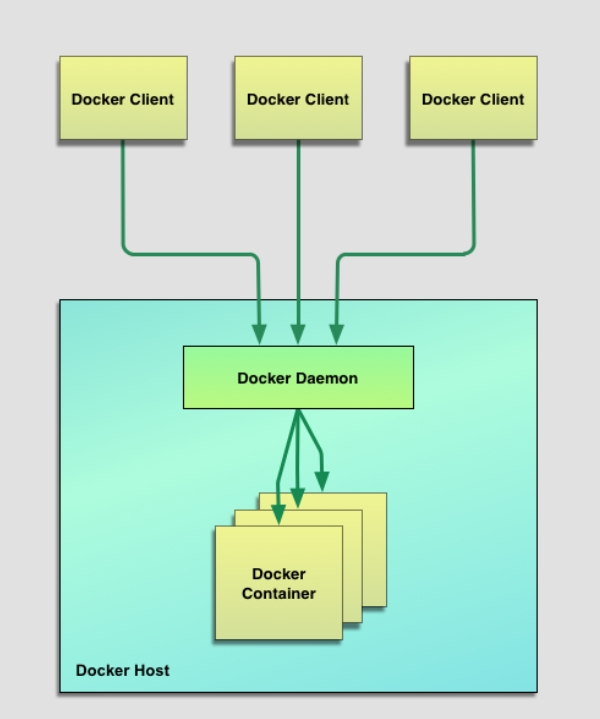
\includegraphics[width=0.9\textwidth]{./images/intro_dockerArchitecture.jpg}
          \caption{Die Client-Server-Architektur von Docker \cite{dockerUnderstandingDocker}.}
          \label{fig:intro_dockerArchitecture}
      \end{figure}

      Der Daemon kann von einer Registry Images (siehe Kapitel \ref{dockerImages} und \ref{dockerRegistries}) beziehen, z.B. dem öffentlichen Docker Hub.
      % Kommunikation zwischen Client und Server via TCPIP oder Unix Sockets?

      Der Docker-Host selbst ist wie in \fig \ref{fig:intro_dockerHost} dargestellt, aufgebaut. Im Idealfall läuft auf der Hardware ein minimales Linux-Betriebssystem, auf dem die Docker-Engine installiert ist. Die Engine verwaltet im Betrieb die Container (siehe Kapitel \ref{dockerContainer}), in denen in \fig \ref{fig:intro_dockerHost} die Apps A-E laufen. Wie auch in der Grafik zu sehen ist, teilen sich die Container gemeinsam verwendete Bibliotheken.% nach der bereits geschilderten \emph{Copy-on-write} Methode.

      \begin{figure}[h]
          \centering
          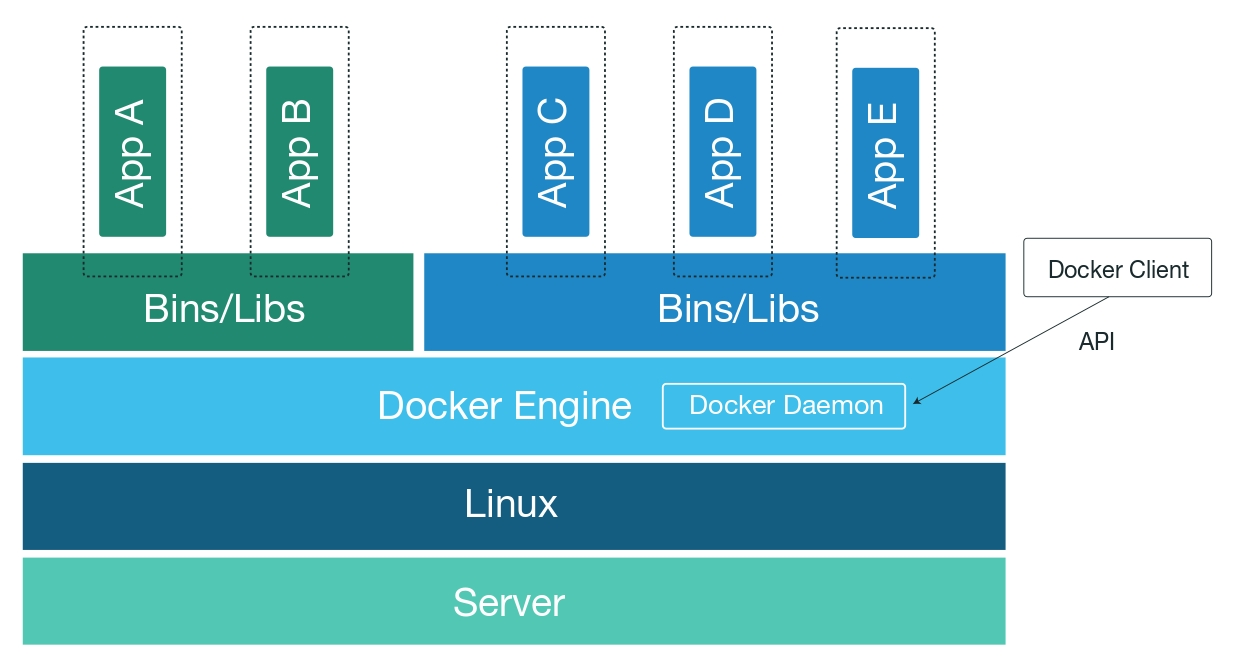
\includegraphics[width=0.9\textwidth]{./images/intro_dockerHost.jpg}
          \caption{Aufbau eines Docker-Hosts, wenn dieser unter einem Linux-Betriebssystem betrieben wird, das direkt auf der Serverhardware läuft. \cite[S.3]{dockerSecIntro}.}
          \label{fig:intro_dockerHost}
      \end{figure}

		\subsection{Dockerfile}
		\label{dockerDockerfile}
      Ein Dockerfile ist eine Datei mit selbigem Namen, die ein oder mehrere Anweisungen enthält. Letztere werden konsekutiv ausgeführt und führen jeweils zu einer neuen Schicht, die in das später generierte Image einfließt. Damit stellen Dockerfiles eine einfache Möglichkeit dar, Images automatisiert zu generieren.

      Eine Anweisung kann z.B. sein, ein Tool zu installieren oder zu starten, eine Umgebungsvariable festlegen oder einen Port zu öffnen. Ein funktionstüchtiges, minimalistisches Dockerfile ist im Folgenden dargestellt und erklärt.

			\begin{lstlisting}
				FROM ubuntu
				MAINTAINER Moritz Hoffmann <mh203@hdm-stuttgart.de>

				RUN \
					apt-get update && \
					apt-get install -y nginx

				WORKDIR /etc/nginx
				CMD ["nginx"]

				EXPOSE 80
				EXPOSE 443
			\end{lstlisting}

			Die Erklärung der einzelnen Anweisungen \cite{dockerDockerfileDocs}:

			\begin{itemize}
				\item \texttt{FROM}: Setzt das Basisimage für alle folgenden Anweisungen. Jedes Dockerfile muss diese Anweisung am Anfang enthalten.
				\item \texttt{MAINTAINER}: Hiermit kann ein Autor des Images festgelegt werden.
				\item \texttt{RUN}: Führt angehängten Befehl während des \gls{Build}vorgangs aus und erzeugt damit eine neue Schicht.
				\item \texttt{WORKDIR}: Setzt das Arbeitsverzeichnis, von dem aus z.B. alle folgenden \texttt{RUN}- und \texttt{CMD}-Anweisungen ausgeführt werden. Kann mehrmals pro Dockerfile vorkommen.
				\item \texttt{CMD}: Führt angehängten Befehl aus, wenn der Container gestartet wird. Pro Dockerfile kann es nur eine \texttt{CMD}-Anweisung geben.
				\item \texttt{EXPOSE}: Öffnet angegebenen Port des Containers zur Laufzeit, in obigem Beispiel Port 80 und 443 für \acrshort{HTTP} und \acrshort{HTTPS}. Gebunden wird dieser standardmäßig auf dem Host auf einen \glqq{}registered\grqq{} Port (1024-49151).
			\end{itemize}

		\subsection{Containerformate \texttt{LXC}, \texttt{libcontainer}, \texttt{runC} und \texttt{OCF}}
		\label{dockerContainerformate}
			Containerformate bilden das Herzstück der containerbasierten Virtualisierung. In ihnen ist in Form einer \acrshort{API} definiert, auf welche Art und Weise Container mit dem Host kommunizieren. Es wird z.B. festgelegt, wie das Dateisystem des Hosts verwendet wird, welche Hostfeatures genutzt werden dürfen und wie die allgemeine Laufzeitumgebung von Containern spezifiziert ist.

			Dockers Containerformat hat sich in den letzten Monaten oft verändert, daher soll an dieser Stelle auf die neusten Entwicklungen eingegangen werden.

			Im ersten Release von Docker wurde die Ausführungsumgebung \emph{LXC} verwendet, die im März 2014 von der \emph{Docker}-eigenen Entwicklung \emph{libcontainer} abgelöst wurde. \emph{libcontainer} ist komplett in der Programmiersprache \emph{Golang} implementiert und kann ohne Dependencies mit dem Kernel kommunizieren \cite{dockerLibcontainer}.

			Ende Juni 2015 hat Docker angekündigt, zusammen mit mehr als 20 Vertretern aus der Industrie, u.a. \emph{Google}, \emph{IBM} und \emph{VMware}, einen neuen Standard \emph{Open Container Format} (\emph{\acrshort{OCF}}) zu schaffen, welcher im Rahmen des \emph{Open Container Project}s (\emph{\acrshort{OCP}}) entstehen soll \cite{dockerOCP}. Am gleichen Tag hat Docker \emph{runC} angekündigt, eine Implementierung des \emph{\acrshort{OCF}}, die maßgeblich auf dem alten Format \emph{libcontainer} beruht, aber die Spezifikationen von \emph{\acrshort{OCF}} umsetzt \cite{dockerRunC}\cite{dockerRunCGithub}\cite{runC}.

		\subsection{Images}
    \label{dockerImages}
			Images bilden als unveränderbare Files die Basis von Containern. Sie sind einfach portierbar und können geteilt, gespeichert und aktualisiert werden. Images sind durch ein \emph{Union}-Dateisystem in Schichten gegliedert, die überlagert ein Image ergeben, das als Container gestartet werden kann \cite[S.11]{dockerBook}. \emph{Union}-Dateisysteme wie \emph{AuFS} und \emph{Device Mapper} haben gemeinsam, dass sie alle auf dem \emph{Copy-on-write}-Modell basieren \cite[S.8]{dockerBook}\cite[S.3]{dockerIntroIEEE}\cite[S.4]{dockerSecIntro}.
			% TODO: Zusatz: "Die Docker alle unterstuetzt (mit Storage Drivern)"

			Genauer gesagt besteht ein Image aus einem Manifest, das auf Datenebene ein oder mehrere Schichten (Layers) referenziert. Images und Schichten sind jeweils über Hashwerte eindeutig refernzierbar und liegen auf dem Docker-Host im Verzeichnis \texttt{/var/lib/docker/graph/}. Im Unterordner eines Images liegen mehrere Image-spezifische Dateien (vgl. \fig \ref{fig:intro_dockerImageVZ}), u.a. das Manifest in der Datei \texttt{json}, das in einer \acrshort{JSON}-Struktur vorliegt und neben Metainformationen auch Details des Dockerfiles, aus dem das Image generiert wurde, beinhaltet \cite{githubDockerGlossary}.

			\begin{figure}[!htbp]
          \centering
          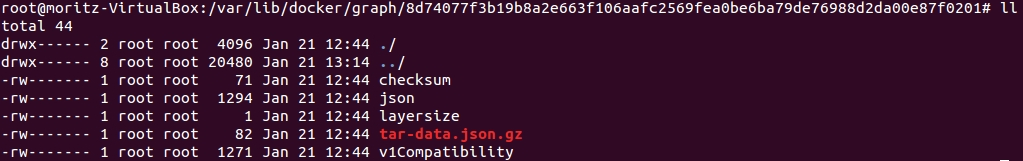
\includegraphics[width=1.0\textwidth]{./images/intro_dockerImageVZ.jpg}
          \caption{Dateien im Ordner eines Images (eigene Abbildung).}
          \label{fig:intro_dockerImageVZ}
      \end{figure}

			Images werden Schritt für Schritt erstellt, z.B. mit den folgenden Aktionen \cite[S.11]{dockerBook}.
			\begin{itemize}
				\item Eine Datei hinzufügen
				\item Ein Kommando ausführen, z.B. ein Tool mittels des Paketmanagers \texttt{apt} installieren
				\item Einen Port öffnen, z.B. den Port 80 für einen Webserver
			\end{itemize}

      Die Schichten eines Images umfassen in der Regel jeweils eine minimale Ausführungsumgebung mit Bibliotheken, Binaries und Hilfspaketen sowie den Quellcode der Anwendung, die im Container ausgeführt werden soll. Die Schichtenstruktur erlaubt es, Images modularisiert aufzubauen, sodass sich Änderungen eines Images zur auf eine Schicht auswirkt. Soll z.B. in ein bestehendes Image der Webserver \emph{Nginx} integriert werden, kann dieser mit dem Kommando \texttt{apt-get install nginx} installiert werden, was eine neue Schicht im Image erzeugt. Eine Auswahl an möglichen Befehlen, die jeweils eine Schicht generieren, ist im Dockerfile-Kapitel \ref{dockerDockerfile} gegeben.

			Mit mehreren ähnlichen Images ist gewährleistet, dass nur die konkreten Unterschiede zwischen diesen als eigene Schichten hinterlegt sind. Eine gemeinsame Codebasis, die von mehreren Images genutzt wird, liegt in wenigen Schichten, die sich die Images teilen \cite[S.3]{dockerIntroIEEE}. Wie in \fig \ref{fig:intro_imagelayers} beispielhaft zu sehen ist, basieren die beiden Images \texttt{redis:3.0.6} und \texttt{nginx:1.9.9} auf zwei gleichen Schichten, die durch die Anweisungen \texttt{ADD} und \texttt{CMD} erzeugt werden. In dieser Abbildung sind die Informationen zu dem Image in der ersten Zeile zu sehen und die Schichten der Images sind in den jeweiligen Spalten vertikal gelistet.
      % Vergleich mit git commit und VCS (S.3 dockerIntroIEEE)

			\begin{figure}[!htbp]
          \centering
          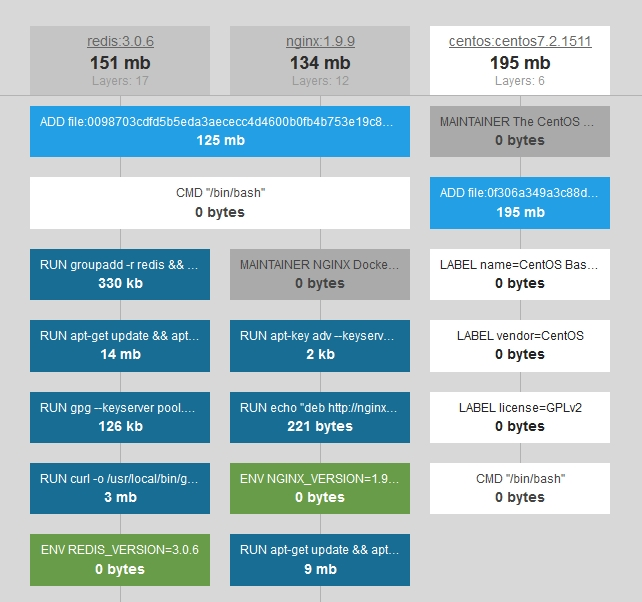
\includegraphics[width=0.8\textwidth]{./images/intro_imagelayers.jpg}
          \caption{Visualisierung eines Vergleichs von Images von \emph{Redis}, \emph{Nginx} und \emph{CentOS} auf Schichtebene \cite{dockerImagelayers}.}
          \label{fig:intro_imagelayers}
      \end{figure}

      % Copy-on-write erklären.

      Über die Kommandozeile kann z.B. das Image eines \emph{CentOS}-Betriebssystems von der öffentlichen Docker-Registry (siehe Kapitel \ref{dockerRegistries}) wie in \fig \ref{fig:intro_dockerPull} mit dem Befehl \texttt{docker pull nginx} auf die lokale Maschine gespeichert werden \cite{dockerHubNginx}\cite{dockerPull}. Wie in \fig \ref{fig:intro_dockerPull} und \fig \ref{fig:intro_imagelayers} zu sehen ist, werden sechs Schichten heruntergeladen, die jeweils über einen Hashwert identifiziert werden und zusammengefügt das angefragte Image \texttt{centos:7.2.1511} ergeben.

			\begin{figure}[!htbp]
          \centering
          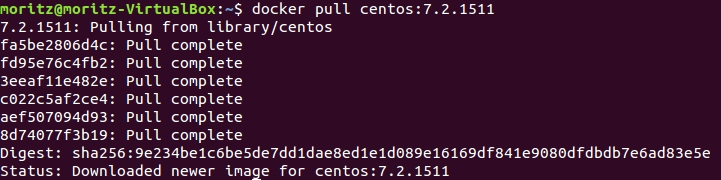
\includegraphics[width=1.0\textwidth]{./images/intro_dockerPull.jpg}
          \caption{Screenshot von der Ausführung des Befehls \texttt{docker pull <image>} (eigene Abbildung).}
          \label{fig:intro_dockerPull}
      \end{figure}

			Eine Liste aller lokal vorliegenden Images, wie in \fig \ref{fig:intro_dockerImages}, kann mit dem Befehl \texttt{docker images} in der Shell generiert werden \cite{dockerImages}.

			\begin{figure}[!htbp]
          \centering
          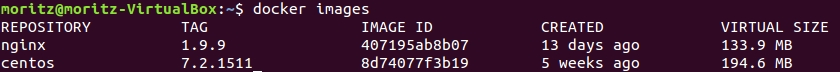
\includegraphics[width=1.0\textwidth]{./images/intro_dockerImages.jpg}
          \caption{Screenshot von der Ausführung des Befehls \texttt{docker images} (eigene Abbildung).}
          \label{fig:intro_dockerImages}
      \end{figure}

			% TODO: Ist Quelle https://docs.docker.com/engine/reference/commandline/images/ hier mit drin - eingearbeitet?

			% Seit registry api version 2 sind images content addressable
			%	Über kryptographisch sichere Hash ...sha256(bytes)
			% einfach und unabhängig verifizierbar
			% leverages merkle DAG ... damit naeher an git
			% weitere Vorteile auf s.21
			% unterschiede zu v1 auf s.23
			% seit docker 1.6 ist registrz v2 im einsatz
			%		^ 	\cite[S.15+16]{http://www.slideshare.net/Docker/docker-48351569}
			%

    \subsection{Container}
		\label{dockerContainer}
      % Metapher mit dem Docker-Wal, der Container lädt: Docker als Frachtschiff, mit dem Container verschifft werden.
			Ein Container ist die laufende Instanz eines Images, die in Sekundenbruchteilen gestartet werden kann \cite[S.1]{dockerIntroIEEE}. Sie beinhalten eine idealerweise minimale Laufzeitumgebung, in der eine oder mehrere Anwendungen laufen.

      In Bezug zu anderen Docker-Begriffen, enthält ein Container ein Image und erlaubt eine Reihen von Operationen, die auf ihn angewandt werden können. Darunter fallen z.B. das Erstellen, Starten, Stoppen, Neustarten und Beenden eines Containers. Welchen Inhalt einen Container hat, also ob ein Container z.B. auf einem Datenbank- oder Webserver-Image beruht, ist dafür unerheblich \cite[S.12]{dockerBook}\cite[S.2]{dockerLXCKub}.

      Ein Container wird als priveligiert bezeichnet, wenn er mit Root-Rechten gestartet wurde. Standardmäßig startet ein Container unpriveligiert ohne Root-Rechte. Mit einem reduzierten Set an ausführbaren Aktionen, die über verschiedenene, in Kapitel \ref{secLinux} vorgestellte Mechanismen definiert werden, lassen sich Container unabhängig von Root-Rechten einschränken.
			% TODO: QUELLE + Verweis auf capabiltiies kapitel? Oder Glossareintrag "capabilities"

      % Der Hosts selbst muss auch gemanaged werden.
      % Docker als Anwendung muss installiert, gemanaged, und deployed werden auf einem Host.
      % Docker-Container müssen orchestriert, gemanged und deployed werden. Oft im Zusammenspiel mit externen Service und Tools.
      % In Hypervisor-basierten Virtualisierungen kommen meist Puppet, Chef )und Vagrant) zum Einsatz, die obigen Management-Anforderungen erfüllen können.
      % Aber beim Einsatz von Docker sind diese Tools nicht unbedingt notwendig,  Docker repräsentiert oft kurzlebige Container, read-only Container, die einfach zu ersetzen sind ohne die Notwendigkeit Containerzustände zu speichern oder wiederherzustellen. Wenn ein Zustand von Bedeutung ist, kann es einfacher sein diesen neu zu erstellen anstatt einen bestehnden Zustand zu korrigieren.
      % ^  \cite[S.14]{dockerBook}

      % In der Praxis werden herkömmliche, oft historisch gewachsene Lösungen nicht vollständig und sofort auf Docker umgerüstet. Mit der Koexistenz von Hypervisor-basierten Virtualisierungen und Containerlösungen, werden auch Configuration Management Tools wie Puppet und Chef im Zusammenhang mit Docker verwendet.
      % ^  \cite[S.14]{dockerBook}

		\subsection{Registries}
		\label{dockerRegistries}
      Eine Registry ist eine Webanwendung, der als Speicher- und Verteilerplattform für Images dient. Über eine wohldefinierte API, die Registry-API, sind Docker-Komponenten in der Lage mit Registries zu kommunizieren. Images sind mit Tags versehen in Repositories gegliedert, die wiederum in der Registry liegen \cite{dockerRegistry}. Ein Repository besteht aus mindestens einem Image.
			% TODO: visit source, and extend registry info here
			% TODO: was zu registry api version 1 und 2, 2.1, 2.2, 2.3 schreiben und bisschen vergleichen
			%		^		\cite{http://www.slideshare.net/Docker/docker-48351569 ... slide 11}\cite{https://docs.docker.com/registry/spec/api/}

      \emph{Docker} stellt eine Vielzahl an Images öffentlich und frei verwendbar in einem Service, dem Docker Hub, zur Verfügung \cite[S.11]{dockerBook}\cite[S.3]{dockerSec1}\cite{dockerRegistry}. Für dieses System können Personen und Organisationen Accounts anlegen und eigenständig Images in öffentliche und private Repositories hochladen. Das Docker-Hub bietet bereits mehr als 150.000 Repositories, die etwa 240.000 Nutzer zusammenstellten und hochluden, zur freien Verwendung an (Stand Juni 2015) \cite[S.16]{slideshareDockercon15}. Wie in \fig \ref{fig:intro_registry} zu sehen ist, werden auch Nutzungsstatistiken pro Image gesammelt und angezeigt. Durch diese erweiternden Features ist das Docker Hub per Definition keine Registry, sondern enthält eine Registry als Teil des Angebotspektrums. % \cite[S.8]{http://www.slideshare.net/Docker/docker-48351569}

      \begin{figure}[h]
          \centering
          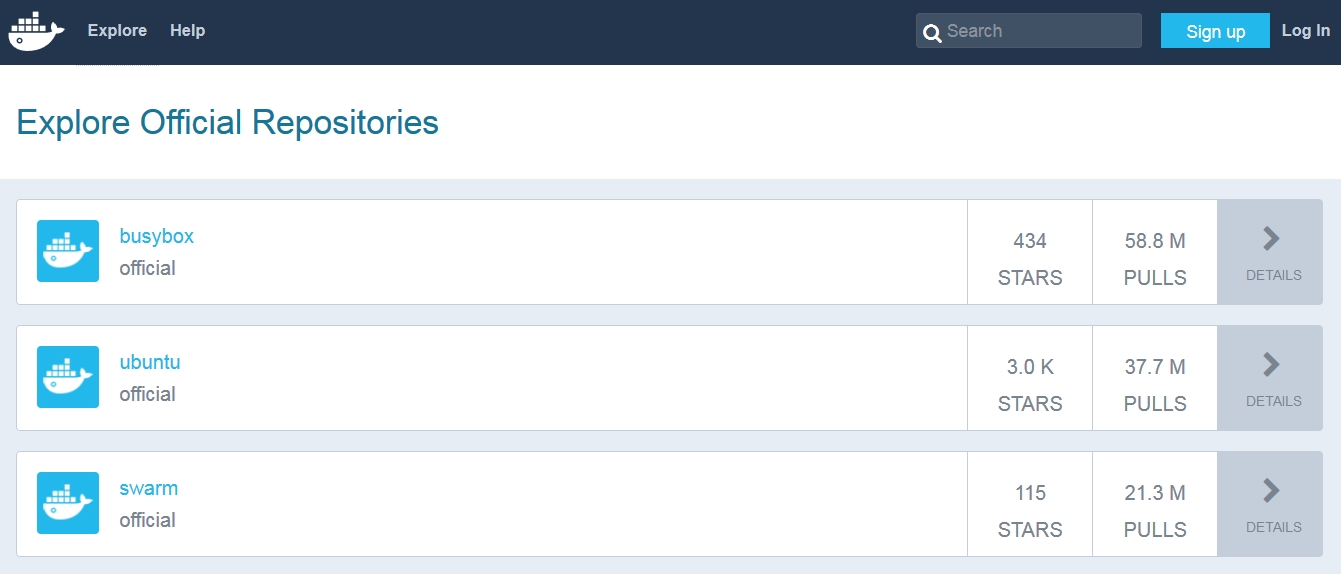
\includegraphics[width=1.0\textwidth]{./images/intro_registry.jpg}
          \caption{Web-\acrshort{UI} des Docker Hubs mit den beliebtesten Repositories \cite{dockerHub}.}
          \label{fig:intro_registry}
      \end{figure}

			Um Images in einem Repository voneinander zu unterscheiden, werden Images Tags zugewiesen, um beispielweise mehrere Versionen eines Images in einem Repository zu kennzeichnen. Die Images werden nach dem Schema \texttt{<repository>:<tag>} identifiziert. So gibt es z.B. im offiziellen Repository des Webservers \emph{Nginx} Images mit den Tags \texttt{latest}, \texttt{1}, \texttt{1.9} und \texttt{1.9.9} \cite{dockerHubNginx}. Wenn bei dem Download kein Tag angegeben ist, wie in Kapitel wird automatisch das aktuellste Image mit dem Tag \texttt{latest} bezogen.

      % es gibt eine Trusted Registry. Die noch erklären.

      % Bsp. geben für z.B. Ubuntu mit vielen Unterversionen und dem Identifier "latest".

      % Weitere beispiele aus dockerBook: Nginx web server, MySQL Datenbank

      % Es gibt offizielle Images, die von trusted parties verwaltet werden

\end{document}
